\chapter{Háttér}
Az emberi arcfelismerés elfogadott modelljég Burce és Young \cite{bruce_understanding_1986} dolgozták ki 1986-ban. A \ref{Bruce_and_Young_face_recognition_model}. ábrán vázolt modellen jól látható, hogy a probléma igen összetett, több alfeladatra osztható, melyek egyenként további lépésekre bonthatóak szét. Első lépésben az érzékelt kép alapján egy első lépés minden esetben az arc strukturális kódolása, mely alapján a különböző felismerési és hozzárendelési feladatok elvégezhetőek.

\begin{figure}
    \centering
    \includegraphics[width=\linewidth]{figures/bruce-young.png}
    \caption{Bruce és Young arcfelismerési modellje. \cite{kornel_az_2015}-ból átemelve.}
    \label{Bruce_and_Young_face_recognition_model}
\end{figure}

Amennyiben ezt számítógépen kívánjuk megvalósítani első lépésben szükségessé válik az adott képen található arcok képen belüli helyzetének meghatározása melyet arcdetekciónak nevezünk. Ezt hozzávéve a modellünkhöz megkapjuk a gépi arcfelismerésben alkalmazott felosztást: arcdetekció, jellemzők kinyerése, majd ezek alapján a felismerés (személyazonosítás, hangulatfelismerés, etc.).

A robot kialakítását, az elvégzendő feladatot és a hardver limitációit tekintve ezen feladatok közül csupán az elsőt, a detekciót kívánjuk elvégezni. A feladatok párhuzamosíthatóságának köszönhetően amennyiben szükségessé válnak és az erőforrások engedik további nodeok hozhatóak létre ezek elvégzésére.

\section{Arcdetekció}

\subsection{Definíció}
"Az arcdetekció célja egy adott tetszőleges képen annak meghatározása, hogy a képen találhatóak-e arcok és amennyiben igen ezek pozíciójának és méretének megadása." \cite{yang_wider_2016} \todo{ide jöhetne az a cikk is, amit a wideresek hivatkoznak}

Ez a gyakorlatban majdnem minden esetben az arcot tartalmazó négyzet alakú terület, ún. bounding box meghatározását jelenti.

\subsection{Irodalmi áttekintés}
Lévén az arcdetekció elsődleges feltétel a különböző arcelemző eljárásokhoz és emellett a vizuális ember-gép és ember-robot interakció alapja lehet, a terület régóta kutattott. Korai munkákat találhatunk akár több mint 50 évvel korábbról is \cite{chan_man-machine_1965,sakai_computer_1972}. A '90-es években számos más kutatási területhez hasonlóan itt is robbanásszerű fejlődés volt tapasztalható \cite{yang_detecting_2002}.

\subsubsection*{Pre-deep-learning korszak}

\paragraph{Viola \& Jones}\hfill

Az első valódi praktikus megoldást azonban Viola és Jones \cite{viola_robust_2004} munkája hozta el. A módszer három kiemelkedő ötletet alkalmazott a valós idejű futás elérésének érdekében: az integrál képet, a figyelem-kaszkádot és az AdaBoost tanulóalgoritmust.

Integrál kép: 
A summed-area table (összesített terület táblázat) használatának ötletét 1984-ben Frank Crow vezette be a számítógépes grafika területén \cite{crow_summed-area_1984} mipmapokban történő alkalmazásra. Az integrál kép elnevezés Viola és Jones munkája folytán vált a módszer elterjedt alternatív elnevezésévé. Az algoritmus a Haar-szerű funkciók gyors számításához használja. Az eredeti képből a következőképpen számolható:
\begin{equation}
    ii(x, y) = \sum_{x' \leq x, y' \leq y} i(x', y'),
\end{equation}
ahol $ii(x, y)$ az integrál kép egy adott $(x, y)$ képpontban, $i(x', y')$ pedig az eredeti kép pixelei. Ebből a képpontok összege a kép bármely ABCD pontok által meghatározott négyszögletű területén (lásd \ref{fig:integral_image_and_haar-like_features}) a következőképp számolható:
\begin{equation}
    \sum_{(x, y) \in ABCD} i(x, y) = ii(D) + ii(A) - ii(B) - ii(C)
\end{equation}
Mivel a Haar-szerű funkciók 2-4 súlyozott négyszögletes területek összegeképp képezhetőek (lásd \ref{fig:integral_image_and_haar-like_features}. ábra) és egy-egy terület kiszámításához így csupán négy darab tömb referencia szükséges a számítás költsége jóval alacsonyabb lesz.

AdaBoost tanulás:
A boostolás névre hallgató metódusok lényege, hogy sok gyenge, közepes pontosságú hipotézis kombinációjaként igyekeznek találni egy magas pontosságú hipotézist. Az eredeti AdaBoost (Adaptive Boosting) \cite{freund_decision-theoretic_1997} algoritmus megnyitotta az utat a későbbi praktikusabb boosting eljárások felé \cite{freund_decision-theoretic_1997}. A diplomamunkának nem célja a boosting eljárások részletesebb ismertetése, amennyiben az olvasó betekintést kíván nyerni a területre Meir és R{\"a}tsc cikke \cite{meir_introduction_2003} jó kezdőpontot szolgáltat.

\begin{figure}
    \centering
    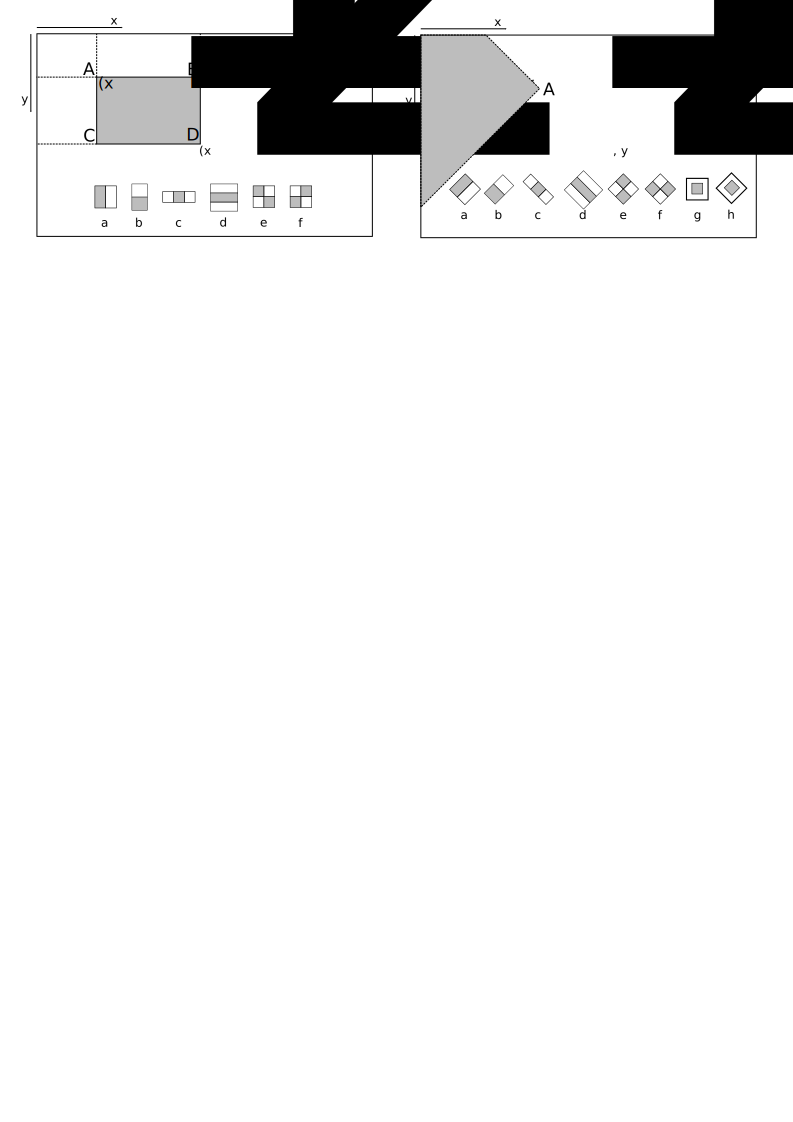
\includegraphics[width=\linewidth]{figures/integral_img_and_haar.png}
    \caption{Bal oldal: Összesített terület táblázat / integrál kép és Haar-szerű funkciók (a-f). Jobb oldal: Példa a későbbi lehetséges kiegészítésekre. Elforgatott integrál kép és két újabb Haar-szerű funkció (g, h).}
    \label{fig:integral_image_and_haar-like_features}
\end{figure}

Figyelmi kaszkád:
A figyelmi kaszkád az integrál képen túl az algoritmus másik sebesség szempontjából kritikus eleme. A megfigyelés lényege, hogy létrehozhatunk olyan gyengébb osztályozókat, melyek a negatív ablakok többségét elutasítják, míg a pozitív ablakokat majdnem mind detektálják. Ennek köszönhetően az összetettebb, nagyobb számításigényű osztályozókat már csak jóval kevesebb részletre kell futtatnunk a benn maradt hamis pozitívok kiszűrésére. Ennek sematikus ábrázolása látható a \ref{fig:attentional_cascade}. ábrán.

\begin{figure}
    \centering
    \includegraphics[width=\linewidth]{figures/attentional_cascade.png}
    \caption{Figyelmi kaszkád}
    \label{fig:attentional_cascade}
\end{figure}

Az eredeti cikkben \cite{viola_robust_2004} a figyelmi kaszkádot kézzel állították össze. Ez azt jelenti, hogy az osztályzók számát és elutasítási küszöbét manuálisan kellett specifikálni. Ez igen nehéz feladat, hiszen amennyiben túl szigorúan állítjuk össze a feltételeket gyors, ám gyenge detekciós rátájú detektort kapunk. Amennyiben az ellenkező irányba térünk ki a detektor ugyan pontos lesz, ám lassú is.

A módszer továbbfejlesztésére nagy mértékű kísérlet irányult. Ezek többnyire a következő módosításokkal álltak elő:

\begin{itemize}
    \item A téglalap alakú jellemzők lecserélése vagy kibővítése valamilyen módon, például az eredeti jellemzők 45 fokos elforgatásával \cite{lienhart_extended_2002}.
    \item Különböző új, optimálisabb tanítási eljárások alkalmazásával.
    \item Különböző formában elrendezett figyelmi kaszkádok alkalmazása (\ref{fig:alternative_attentional_cascades}).
\end{itemize}

\begin{figure}[h]
    \centering
    \includegraphics[width=\linewidth]{figures/alternative_cascades.png}
    \caption{Alternatív figyelmi kaszkád struktúrák. A szaggatott nyilak az elutasítást, míg a folytonosak az elfogadást jelzik. a: parallel kaszkád\cite{bo_wu_fast_2004} b: detektor-piramis \cite{goos_statistical_2002}}
    \label{fig:alternative_attentional_cascades}
\end{figure}
\todo{ehhez az ábrához még tudnék szedni alternatívákat és hivatkozásokat}
\todo{egybevonni a sima figyelmi kaszkád ábrát és ezt}

\paragraph{Konvolúció a képfeldolgozásban}\hfill

A képfeldolgozás egyik legfontosabb eszköze a képtérbeli konvolúciós művelet. A módszer lényege, hogy egy konvolúciós ablaknak nevezett mátrix segítségével súlyozva összegezzük a pixelünket a környezetével. Középpontos ablakot feltételezve ez képpontonként a következő módon számítható:
\begin{equation}
    G(i,j) = (I * K)_{ij} = \sum_{u = -m}^{m} \sum_{b = -n}^{n} I(u, v) K(i - u, j - v)
\end{equation},
ahol
\begin{itemize}
    \item \(G(i,j)\) a konvolúció eredménye az \((i, j)\) pontban
    \item \(I(i, j)\) a kép \((i, j)\) pixelének értéke
    \item \(K(i, j)\) a konvolúciós ablak \((i, j)\)-ik értéke
    \item \(m\) a konvolúciós ablak szélességének fele lefelé kerekítve
    \item \(n\) a konvolúciós ablak szélességének fele lefelé kerekítve
\end{itemize}

\begin{figure}[h]
    \centering
    \includegraphics[width=0.5\linewidth]{figures/2D_Convolution.png}
    \caption{Konvolúció képeken.}
    \label{fig:2d_convolution}
\end{figure}

A művelet elvégzésének vizuális magyarázata sokkal intuitívabb. Tegyük fel, hogy a konvolúciós ablakot az
\ref{fig:2d_convolution}. ábra
szerint a képünk bal felső sarkára helyezzük, majd az egy helyre került értékeket összeszorozzuk és a szorzások eredményét összeadva beírjuk az eredményül kapott képünk bal felső sarkába. Ez után az ablakot egy sorral jobbra helyezve a műveletet megismételjük és az eredményt beírjuk az előzőtől egyel jobbra. Mikor egy adott soron végigérünk ugrunk a következő sor elejére, melynek eredményeit a kimenetünk következő sorába írunk. Az ábrán látható, hogy így az eredetihez képest m+1 pixellel keskenyebb és n+1 pixellel alacsonyabb kimenetet kapunk. Ennek kiküszöbölésére paddinget (tömés, bővítés) szokás alkalmazni, mely lényegében egy valamilyen módon megválasztott kiegészítés, keret a képünk számára. Bizonyos esetekben azonban kívánatos lehet a dimenziócsökkentés, ilyenkor megtehetjük, hogy az ablakot több soronként "ugráltatjuk". Ezt a mértéket stridenak (lépcsőzés) nevezik.

Konvolúcióval számtalan képfeldolgozási feladat végezhető el, például szűrések, simítások és különböző irányú éldetektálás.
\todo{opcionálisan ábra}

\paragraph{Histogram of Oriented Gradients (HoG)}\hfill

Bár az irányított gradiensek módszerének ötlete jóval az ezredforduló előttről származik\cite{william_t_freeman_orientation_1994,mcconnell_method_1986}, népszerűvé Dalal és Triggs\cite{dalal_histograms_2005} gyalogosfelismerő módszerének 2005-ös publikálása után vált. Amennyiben a képre \(f(x, y)\) kétváltozós folyamatos függvényként tekintünk annak gradiens vektorát a következő módon számíthatjuk:
\begin{equation}
    \nabla f = |\overline{\nabla f}| = \sqrt{\left(\frac{\partial f}{\partial x}\right)^2 + \left(\frac{\partial f}{\partial y}\right)^2} \approx \left| \left(\frac{\partial f}{\partial x}\right) + \left(\frac{\partial f}{\partial y}\right) \right|
\end{equation}
Digitális képeken ezt a következőképp közelíthetjük:
\begin{equation}
    \nabla f = 
    \begin{bmatrix}
        \frac{\partial f}{\partial x} \\
        \frac{\partial f}{\partial y}
    \end{bmatrix}
    =
    \begin{bmatrix}
        \delta x \\
        \delta y
    \end{bmatrix}
    \approx
    \begin{bmatrix}
        \Delta x \\
        \Delta y
    \end{bmatrix}
\end{equation}
A vektor irányát pedig a következezőképp kaphatjuk meg:
\begin{equation}
    \alpha (x,y) = \arctan \left(\frac{\delta x}{\delta y}\right)
\end{equation}

Az eredeti cikkben több különböző konvolúciós maszkot is teszteltek ennek számítására különböző mértékű Gauss-simítást követően. A legjobbnak az egyszerű \([-1, 0, 1]\) és transzponáltja bizonyultak. A képünket ezután valamilyen stragégia szerint cellákra osztjuk. A vektorokat átváltjuk polárkoordinátákra és a gradiensek terét szög szerint valahány tárolóra osztjuk. Ez után a tárolókat cellánként hisztogram szerűen feltöltjük, azonban a vektorok száma helyett azoknak hosszát adjuk az adott tárolókhoz. Az eredeti cikkben az ellentétes irányú grádiensek egybevonása, tehát a szögek 0 és 180\textdegree közé korlátozása bizonyult, 9 tárolóval. Mivel ez nem túl nagy szám előfordulhat, hogy egy határon lévő grádiens rossz tárolóba kerülne. Ennek kiküszöbölésére érdemes lehet valamilyen stratégia mentén a szomszédos tárolókhoz is hozzáadni annak súlyozott értékét, vagy fuzzy viselkedést vinni a rendszerbe\cite{salhi_histograms_2013}. Ez után a végső HoG jellemzőnket két lépcsős normalizálás után kapjuk. A két lépcső oka, hogy a hisztogramunkat normalizálnunk kell az azonos tárgyat tartalmazó képek közötti kontrasztkülönbségek kiküszöbölésének érdekében. Más részről az gradiensek mértéke egy területen információtartalmat hordoz. Ezért a cellákat először blokkokra osztjuk a teret konvolúciós viselkedés szerint kicsempézve, majd ezeket normalizáljuk. Az euklideszi norma például jó normának bizonyult erre a célra:
\begin{equation}
    b \leftarrow \frac{b}{\sqrt{\Vert b \Vert^2 + \epsilon}}
\end{equation}
\(\epsilon\)-ra a 0 gradiensű blokkok esetén a 0-val való osztás kiküszöbölése miatt van szükség. Ezt követően a kapott eredményeket összefűzzük a végleges HoG jellemzővektorunkba és újra normalizáljuk. A tapasztalat azt mutatja, hogy ebben a lépésben érdemes még egy kiegészítő lépésként visszavágni a kapott nagyon nagy \(h_n\) grádiens eredményeket, mert azok elnyomnák a többit. Ezt követően újra normalizálnunk kell, tehát a folyamat három lépcsőből áll:
\begin{equation}
    \begin{split}
    h \leftarrow \frac{h}{\sqrt{\Vert h \Vert^2 + \epsilon}}\\
    h_{n} \leftarrow \min (h_{n}, \tau)\\
    h \leftarrow \frac{h}{\sqrt{\Vert h \Vert^2 + \epsilon}}
    \end{split}
\end{equation}

A kapott jellemzőteret ez után tetszőlegesen választott klasszifikátorral osztályozhatjuk.

\subsubsection*{Deep learning korszak}
"Az adat az új olaj" - jelentette ki Steve Humby brit matematikus 2006-ban. Amennyiben a ma uralkodó nagyvállalatok profilját tekintjük kijelenthető, hogy állításávan nem tévedett.

Az ezredforduló után a számítási és tárolókapacitás növekedésével, emellett az internet terjedésének köszönhetően robbanásszerűen gyarapodó rendelkezésre álló adatmennyiségnek köszönhetően számos új számítógépes és információtudományi terület látott napvilágot vagy éppen kapott új erőre. Így van ezzel a gépi tanulás mesterséges neurális hálózatokkal foglalkozó területe is. Míg az ezredforduló környékén a Gabor filterek és Support Vector Machineok (SVM) voltak népszerűek és a mai napig használt módszerek, az utóbbi évtizedben a különböző mesterséges neurális hálózatokkal foglalkozó publikációk száma exponenciális növekedésnek indult. Ez jól megfigyelhető a Dimensions\cite{noauthor_dimensions_nodate} \ref{fig:neural_network_article_numbers}. ábrán látható adatain is.

\begin{figure}
    \centering
    \begin{subfigure}[b]{0.45\linewidth}
        \includegraphics[width=\linewidth]{figures/dimensions_ai_artificial_neural_network_publications.png}
        \caption{Publikációk száma}
    \end{subfigure}
    \begin{subfigure}[b]{0.45\linewidth}
        \includegraphics[width=\linewidth]{figures/dimensions_ai_artificial_neural_network_citations.png}
        \caption{Hivatkozások száma}
    \end{subfigure}
    \caption{Mesterséges neurális hálózatokkal foglalkozó publikációk és hivatkozások száma évekre lebontva.}
    \label{fig:neural_network_article_numbers}
\end{figure}

Ez három fő összetevőnek köszönhető. Az első, hogy a felügyelt tanulási módszer magasszintű adatszükséglete egyre több területen biztosított. A második, hogy a számító egységek és a memória növekedésével egyre gyorsabban és egyre nagyobb hálókat tudunk betanítani. Harmadik pedig az ezek hatására elindult kutatások folyamán megalkotott gyorsabb és pontosabb algoritmusok és könyvtárak nem csak jobb eredményeket tesznek lehetővé, de gyorsabb iterációs sebességet is biztosítanak a fejlesztés során.
\todo{ide még lehetne írni arról, hogy az MI és a deep learning diszruptív technológia}

\todo{ehelyett a bekezdés helyett valami értelmeset írni...}
A mesterséges neurális hálózatok és tanításuk részletes ismertetése messze meghaladja ezen diplomamunka kereteit. Amennyiben az olvasó bevezetést kíván nyerni a területre a Deeplearning.Ai\cite{noauthor_deeplearningai_nodate} kurzusai jó kezdőpontot nyújthatnak. Még ha a témát az objektum- vagy akár az arcdetekció témakörére is csökkentjük, a rendelkezésre álló anyagból akár könyvsorozatot is írhatnánk. Ezen okokból most csupán a későbbiekben ismertetett struktúrák megértéséhez minimálisan szükséges eszközkészlet ismertetésére térek ki.

\section{Arcdetekciós benchmarkok}

\subsection{Arcok a vadonban}
Az évek során a különböző arcdetekciós és arcfelismerési eljárások kutatásához és teszteléséhez számos adatszett jelent meg. Azonban a Labeled Faces in the Wild (LFW) megjelenéséig ezeket többnyire jól kontrollált kondíciók között készült képekből állították össze, hogy valamilyen jól specifikált paramétert vizsgálhassanak az arcdetekciós/felismerési területen\cite{huang_labeled_2008}. Ez volt az első megoldás, melynek direkt kitűzött célja a szabad környezetben történő arcfelismerési probléma vizsgálatára szolgáló adatszett nyújtása volt. Ennek köszönhetően az ilyen felállásra legtöbbször az "arcok a vadonban" koncepcióként referálnak. Mára ilyen típusú adatszettek közül kerülnek ki a legnépszerűbbek mind tanítási, mind kiérékelési célokra.

\todo{ide kell kép?}

\subsection{A detekció kiértékelése}
\todo{kell ez? lényegében az IoU-t tudnám leírni ide}

\subsection{FDDB}
2010-ben, az "FDDB: A Benchmark for Face Detection in Unconstrained Settings" \cite{jain_fddb_2010} cikkel nyilvánosságra hozott adatbázis. 2845 képből áll, összesen 5171 felcímkézett arcot tartalmaz. Létrehozásának célja a korábbi létező adatszettek problémáinak kiküszöbölése és protokoll bizosítása az arcdetekciós megoldások összehasonlítására. Alapját a Berg és munkatársai által a Yahoo news 
\todo{Az oldalt ilyenkor be kell hivatkozni?} 
híroldalról származó videókból összeállított adatbázis képzi. Mivel az eredeti sok közel azonos képet tartalmazott első lépésben ezeket 103 csoportba klaszterezték 
\todo{ez amúgy valid szó?}, 
majd mindegyik csoporból egy képet tartottak meg. Ezt követően minden arcot előzetesen felcímkéztek, melynek mérete meghaladta a 20 pixelt. Az alacsony felbontásból, megvilágításból és pozícióból adódó bizonytalanságok kiszűrésére ezután minden képet több emberrel felcímkéztettek egy webes felületen keresztül. Ezen lépésig a szerzők bounding boxokat (dobozokat / négyzet alakú jelölőket) alkalmaztak. A megmaradt arcok dobozait ezek után ellipszisekre cserélték le, mert úgy vélték ez jobb reprezentációja az arcoknak.

\subsection{AFW}
A “Face Detection, Pose Estimation and Landmark Localization in the Wild” \cite{zhu_face_2012} című cikk részeként létrehozott "annotált arcok a vadonban" (annotated faces in-the-wild) adatszett célja a papírban prezentált egyidejű arcdetekciót, pózbecslést és jellemzőkinyerést végző algoritmus kiértékeléséhez egy új, az arcok a vadonban elvet követő megoldást biztosítsanak.

205 Flickr-ről\cite{noauthor_flickr_nodate} származó képet tartalmaz, ezeken összesen 468 annotált arc található. A címkék tartalmazzák az arcot körülvevő dobozt, 6 jellemző pontot és három további, az arc orientációját leíró számot.

A szerzők állítása alapján a képek zsúfolt háttereket és mind megjelenésben, mind pózban változó arcokat tartalmaznak, bár ezek mértéke nincs külön számszerűsítve.

\subsection{PASCAL Face}
A "Face detection by structural models" \cite{yan_face_2014} szerzői az előző két adatszetten túl a Pascal VOC \cite{everingham_pascal_2010} objektumdetekciós és kategorizációs kihívás adatainak arcokra történő szűkítésével egy új mércét is alkalmaztak.

851 képet tartalmaz, ezeken 1335 nagyban különböző arc található (bár a különbözőség itt sincs számosítva). A jelölések és a kiértékelési módszer megegyezik a Pascal VOC-al.

\subsection{WIDER FACE}
Az arcdetekció nagy erővel kutatott területén tapasztalható előrelépések jelentős részben a különböző gépi tanulási módszerekben történő előrelépéseknek köszönhetőek. Jelenleg a mélytanulási eljárással tanított neurális hálózatok uralják a területet. Ezek adatigényességéből kiindulva nem meglepő, hogy az előrelépések nagymértékben az elérhető egyre bővebb és részletesebb adatszetteknek köszönhetőek. Ezen a vonalon gondolkodva jött létre a 2016-ban publikált "WIDER FACE: A Face Detection Benchmark" \cite{yang_wider_2016} adatszett. Publikálásakor az akkoriban elérhető egyéb megoldásokhoz képest nagyságrendbeli növekedést jelentett mind a képek száma, mind az annotált arcok száma tekintetében. Emellett az egy ével korábban publikált MALF \cite{bin_yang_fine-grained_2015} adatkészlet után a második olyan megoldás, mely részletesebb címkéket biztosít a részletesebb kiértékeléshez (és tanításhoz) az arcok pozícióját és takarását illetően. A MALF szetthez képest továbbá a képen látható eseményekkel kapcsolatos címkék is rendelkezésre állnak.

Az adatszett a WIDER eseményfelismerő adatkészlet része, amely 60 különböző eseményből áll. Az esemény kategóriákat a "Large-Scale Concept Ontology for Multimedia" (LSCOM) \cite{naphade_large-scale_2006} elveit követve, illetve diákok véleményét figyelembe vége alkották meg. Ezt követően különböző keresőmotorok használatával kategóriánként 1000-3000 képet gyűjtöttek össze.

A WIDER FACE létrehozásához ezután manuálisan eltávolították az arcokat nem tartalmazó képeket és a diverzitás biztosítása érdekében a hasonló képeket egyet-egyet kivéve eltávolították. Az annotáció során a dobozokat úgy állították be, hogy azok tartalmazzák a homlokot, az állat és az orcákat. A homályosság vagy kis méret (10 pixel alatt) miatt nehezen felismerhető arcokat 'ignore' (figyelmen kívül hagy) címkével látták el. Ezen kívül az arcok pozíciója szempontjából 'typical' (tipikus) és 'atypical' (nem tipikus), kitakartságuk szempontjából pedig 'none' - 'partial' - 'heavy' (nincs - részleges - erős) címkéket hoztak létre. A részleges és erős címkék 1-30\%-os és 30\% feletti takarást jelentenek. Ezeken kívül 'expression' (kifejezés), 'illuminaiton' (megvilágítás) és 'blur' (elmosódottság) címkék is rendelkezésre állnak, bár ezeket a cikk nem részletezi. Az eredeti annotátoron kívül minden címkét két további ember ellenőrzött.

A teljes szettet EdgeBox \cite{zitnick_edge_2014} algoritmust alkalmazva a különböző események detekciós rátáját figyelembe véve könnyű, közepes és nehéz részekre osztották szét. Ezen kívül annak érdekében, hogy az adatok tanításra is felhasználhatóak legyenek véletlenszerűen tanító, validációs és teszt részekre osztották 40\% / 10\% / 50\% arányban. Emellett a cikkben említik, hogy az arcok mérete szerint is szeparálhatóak az adatok, általuk ajánlottan 10-50, 50-300 és 300 feletti méretekre, azonban ezt szükség esetén a dobozok magasságát tekintve sajátkezűleg kell elvégezni.

A képek, a tanító és validációs részek címkéi a WIDER FACE hivatalos oldaláról \cite{noauthor_wider_nodate} bárki számára letölthetőek. A teszt szetten történő kiértékeléshez jelenleg az eredményeket a szerzőknek kell elküldeni, az oldal szerint a közeljövőben automatikus kiértékelésre webszerver készül. A 2016-os publikációt figyelembe véve ezen állítás igazságtartalma kétségbe vonható.

Ennek ellenére amennyiben a teljes adatmennyiség felét tekintjük rendelkezésre állónak, akkor is jelentős méret, nehézség és részletességbeli javulást jelent a korábi népszerű benchmarkokhoz képest. Ezen kívül a tanító- és validációs felosztás rendelkezésre állását tekintve nem meglepő, hogy a WIDER FACE az egyik legnépszerűbb napjainkban elérhető adatszett.

\begin{table}[!ht]
    \footnotesize
    \centering
    \renewcommand{\arraystretch}{1.5}
    \begin{tabular} {|l | c | c |l |}
        \hline
        Név & Protokoll & Annotáció részletessége & Kód \\
        \hline \hline
        FDDB & ROC & Alacsony & Python 2.7 kiértékelő kód, konténerben futtatható \\
        \hline
        AFW & PASCAL VOC & Alacsony & Nem hivatalos Python kód \\
        \hline
        PASCAL Face & PASCAL VOC & Alacsony & Nem hivatalos Python kód \\
        \hline
        WIDER Face & PASCAL VOC & Magas & Matlab kód ellenőrzéshez \\
        \hline
    \end{tabular}
    \caption{Arcdetekciós adatszettek összefoglaló táblázata}
    \label{tab:arcdetekcio}
\end{table}

\section{ROS}
Nevével ellentétben a Robot Operating System (Robot Operációs Rendszer, ROS) nem operációs rendszer, hanem egy robotspecifikus middleware (köztes szoftver), mely 2007-ben a Stanford Egyetem Personal Robotics Program (Személyes Robot Program)\cite{noauthor_stanford_nodate} keretein belül jött létre az ugyan azon az egyetemen futó STAIR\cite{noauthor_stair_nodate} program keretein belül fejlesztett kódbázisra épülve. 2007-2013 között a Willow Garage, majd 2013-ban az Open Source Robotic Foundation (OSRF)\cite{noauthor_open_nodate} vette át a kezelését. Ettől a ponttól kezdve évi rendszerességgel adtak ki új verziókat. Mára projektek ezrei alkalmazzák és élénk fejlesztői közösség veszi körül. 2014-es bejelentése óta párhuzamosan fut a modernebb technológiára épülő és szignifikáns különbségekkel rendelkező ROS 2 fejlesztése is, ennek elterjedtsége azonban még elődjénél kisebb. A ROS konceptuálisan három szintre bontható: fájlrenszer, komputációs gráf és közösség.

\subsection{Fájlrendszer}
Ez a szint a ROS elrendezését takarja a háttértáron, melynek alapvető atomi szervezési egysége a csomag, ez a legkisebb önálló rész, melyet a ROS-ban létrehozhatunk. A csomag lényegében egy feladatkört ellátó vagy valamilyen más módon kapcsolódó programok és a hozzájuk szükséges adatok összessége. Ennek célja, hogy a szoftver újra felhasználható legyen más projektekben. A csomagokhoz manifesztumok (\lstinline{manifest.xml}) tartoznak, melyek metaadatokat szolgáltatnak a csomagról, mint például annak neve, karbantartója, licensze és más csomagoktól való függősége(i). Létrehozhatunk csomagokat összefogó metacsomagokat is, melyek többnyire konceptuális szinten összekapcsolódó programcsoportokat képeznek. Jó példa erre a mobil robotok navigációjához haszált Navigation stack\cite{noauthor_navigation_nodate}, de metacsomagba rendezhetjük például a robotunk szimulációjához szükséges csomagokat is. Ennek köszönhetően egy szabadon választott verziókezelő rendszerrel és megosztófelülettel - például Git\cite{noauthor_git_nodate} és Github\cite{noauthor_github_nodate} - könnyedén oszthatunk meg és fejleszthetünk komplett programcsomagokat.

Csomagjaink tartalmazzák továbbá az egyes programrészek közötti kommunikációra használt message (msg, üzenet) és service (srv, szolgáltatás) üzenettípusok definícióit. Egy csomag általános felépítése a \ref{fig:ros_package_structure}. ábrán látható.

\begin{figure}
    \centering
    \framebox[\textwidth]{
    \begin{minipage}{0.9\textwidth}
    \dirtree{%
    .1 catkin\_ws.
    .2 src.
    .3 CMakeLists.txt.
    .3 package\_1\_name.
    .4 CMakeLists.txt.
    .4 package.xml.
    .4 launch\DTcomment{indító fileok}.
    .5 \dots .
    .4 msg.
    .5 message\_name.msg.
    .5 \dots .
    .4 scripts\DTcomment{Python scriptek}.
    .5 \dots .
    .4 src\DTcomment{Forráskódok (C++, esetleg Python)}.
    .5 \dots .
    .4 srv.
    .5 service\_name.srv.
    .5 \dots .
    .4 \dots \DTcomment{a csomag működéséhez szükséges egyéb fileok}.
    .3 \dots \DTcomment{a többi csomag, hasonló struktúrával}.
    }
    \end{minipage}
    }
    \caption{Egy ROS csomag általános felépítése. A csomagon belül tetszőleges számú további mappát és filet elhelyezhetünk, mely annak működéséhez vagy forráskódból fordításához szükséges.}
    \label{fig:ros_package_structure}
\end{figure}

\subsection{Komputációs gráf}
Komputációs gráf alatt a ROS által megvalósított peer-to-peer (egyenrangú) kommunikációs hálózatot értjük. Elemei a nodeok, topicok, messagek, servicek, a paraméterszerver és a master. A nodeok a futó programjainkat takarják, melyek topicokra iratkozhatnak fel információért, ezen számításokat végezhetnek és az eredményt szükség esetén szintén topicokra publikálhatják. Egy csomag több nodeot is tartlamazhat, melyek így kommunikálva akár több lépésen keresztül is megoldhatnak egy összetett feladatot. A kommunikáció üzenetek segítségével történik. Az üzenet egy adatszerkezet, mely típusos mezőkből áll. A jellemző primitív típusok (egész és lebegőpontos számok, logikai értékek, karakterek, stb.) és ezek tömbjei is támogatottak. Emellett a C structjaihoz hasonlóan tetszőleges egymásba ágyazott típusokat is felépíthetünk a primitív típusokból.

Az üzenetek továbbítására két különböző megoldás áll rendelkezésre. Az első a topicok (témák) alkalmazása. A kommunikácó feliratkozásokon és publikációkon keresztül folyik. Amennyiben egy nodenak szüksége van valamilyen információra, feliratkozhat annak topicjára, szabadon hozzáférve a mások által oda publikált tartalomhoz. A feliratkozók és publikálók száma nincs lekorlátozva, tehát a kommunikáció many-to-many (sokan sokfelé). Amennyiben egy az egyhez kommunikációt kívánunk megvalósítani service(ke)t (szolgáltatás) kell alkalmaznunk. Ezeket egy message-pár definiálja, mellyel kérdés-válasz típusú kommunikációt valósítanak meg.

Az egyes nodeok neveinek regisztrációját és azok megtalásának biztosítását a ROS Master végzi, melyet egy DNS szerverhez hasonlíthatunk. A Master része továbbá a Paraméterszerver, mely központi kulcsalapú adattárolást tesz lehetővé. A leírtakat megvalósító \lstinline{ros_comm}\cite{noauthor_ros_comm_nodate} csomag tartalmazza emellett még a rosbagek (zsákok) implementációját, melyek az üzenetek tárolására és visszajátszására használhatóak. A komputációs gráf sematikus ábrája a
\ref{fig:computational_graph}. ábrán látható.

\begin{figure}
    \centering
    \begin{subfigure}[b]{0.45\linewidth}
        \includegraphics[width=\linewidth]{figures/computational_graph.png}
        \caption{Sematikus ábra}
    \end{subfigure}
    \begin{subfigure}[b]{0.45\linewidth}
        \includegraphics[width=\linewidth]{figures/ros_rqt_graph.png}
        \caption{rqt\_graph}
    \end{subfigure}
    \caption{A komputációs gráf szemléltetése. Bal oldal: sematikus ábra a leírtakról. Jobb oldal: a ROS beépítet \lstinline{rqt\_graph} eszközének kimenete egy egyszerű példán. Oválisok - nodeok, négyszögek - topicok. A \lstinline{turtle1} nagy négyszög egy névteret jelez, mellyel összetartozó topicokat csoportosíthatunk.}
    \label{fig:computational_graph}
\end{figure}

Az így megvalósított rendszer előnye, hogy független végrehajtást tesz lehetővé az alegységek között. Ez azt jelenti, hogy a topicok neveinek egyeztetésével különböző szenzoros és feldolgozó egységek csatolhatóak egymáshoz. Ez azért lehetséges, mert a nevek terminálon keresztül történő újradefiniálását minden ros klienskönyvtár beépítetten támogatja. Így például amennyiben megvalósítunk egy gyorsabb arcfelismerésre képes nodeot az azt megelőzőt könnyűszerrel leválthatjuk. 

A kommunikációhoz használt protokoll legtöbbször a TCPROS\cite{noauthor_rostcpros_nodate}, mely standard TCP/IP socketeket használ, így a robot részei közötti kommunikáció mellett robot-robot kommunikáció is könnyen megvalósítható.

\subsection{Közösségi szint}

A ROS alapvetően szabad szoftver\cite{noauthor_what_nodate}, bár a pontos licenszelése könyvtáranként változó és mint az ilyeneknél jellemző, fejlesztésének jelentős része közösségi alapon folyik. A közösségi szint a különböző ROS disztribúciókat,  repositorykat, a ROS Wikit\cite{noauthor_ros-wiki_nodate}, a ROS Discourse fórumot\cite{noauthor_ros-discourse_nodate}, a ROS Answers Q\&A oldalt\cite{noauthor_ros-answers_nodate} és levelezési listákat. A felsoroltak célja, hogy lehetővé tegyék a különböző szoftverek, tudás és ötletek cseréjét a fejlszetőcsoportok, kutatók és hobbiisták között. A ROS disztribúciói a Linux disztribúciókhoz hasonlóan verziószámmal ellátott szoftvercsomagokat jelentenek, melyek lehetővé teszik, hogy a felhasználók egy tesztelt és működő kódbázisra építhessék projektjeiket. Ennek köszönhetően egy újabb ROS verzió megjelenése esetén is az előző verzió(ka)t használva tovább működhetnek a rá épülő applikációk, időt adva a független fejlesztőknek kódbázisuk frissítésére.

A közösségi részvétel maximalizálása érdekében a ROS föderált tároló modellt követ. Ez azt jelenti, hogy a felhasználókat és a fejlesztőket arra ösztönzik, hogy ROS-csomagjaikhoz saját maguk üzemeltessék tárolóikat. Így a tárolókat karbantartóik tetszés szerint licenszelhetik és kezelhetik, megtartva a kód tulajdonjogát.

A fejlesztés során a leghasznosabb oldalak a ROS Wiki és a ROS Answers. Az elsőn a fejlesztők projektjeik népszerűsítéshez és dokumentációjához hozhatnak létre oldalakat, így igen részletes katalógust biztosít, mikor különböző feladatokat ellátó csomagokat keresünk. A a Stack Overflowhoz hasonló második egy Q\&A (Kérdés és Válasz) típusú oldal, melyen számtalan gyakran felmerülő problémára találhatunk választ és amennyiben ez nem sikerül magunk is feltehetünk kérdéseket.